\PassOptionsToPackage{unicode=true}{hyperref} % options for packages loaded elsewhere
\PassOptionsToPackage{hyphens}{url}
%
\documentclass[]{scrartcl}
\usepackage{lmodern}
\usepackage{amssymb,amsmath}
\usepackage{ifxetex,ifluatex}
\usepackage{fixltx2e} % provides \textsubscript
\ifnum 0\ifxetex 1\fi\ifluatex 1\fi=0 % if pdftex
  \usepackage[T1]{fontenc}
  \usepackage[utf8]{inputenc}
  \usepackage{textcomp} % provides euro and other symbols
\else % if luatex or xelatex
  \usepackage{unicode-math}
  \defaultfontfeatures{Ligatures=TeX,Scale=MatchLowercase}
\fi
% use upquote if available, for straight quotes in verbatim environments
\IfFileExists{upquote.sty}{\usepackage{upquote}}{}
% use microtype if available
\IfFileExists{microtype.sty}{%
\usepackage[]{microtype}
\UseMicrotypeSet[protrusion]{basicmath} % disable protrusion for tt fonts
}{}
\IfFileExists{parskip.sty}{%
\usepackage{parskip}
}{% else
\setlength{\parindent}{0pt}
\setlength{\parskip}{6pt plus 2pt minus 1pt}
}
\usepackage{hyperref}
\hypersetup{
            pdftitle={Supplementary Material for The Joint Evolution of Movement and Competition Strategies},
            pdfauthor={Pratik R. Gupte; Christoph F.G. Netz; Franz J. Weissing},
            pdfborder={0 0 0},
            breaklinks=true}
\urlstyle{same}  % don't use monospace font for urls
\usepackage[left=3cm, right=3cm, top=2.5cm, bottom=2.5cm]{geometry}
\usepackage{longtable,booktabs}
% Fix footnotes in tables (requires footnote package)
\IfFileExists{footnote.sty}{\usepackage{footnote}\makesavenoteenv{longtable}}{}
\usepackage{graphicx,grffile}
\makeatletter
\def\maxwidth{\ifdim\Gin@nat@width>\linewidth\linewidth\else\Gin@nat@width\fi}
\def\maxheight{\ifdim\Gin@nat@height>\textheight\textheight\else\Gin@nat@height\fi}
\makeatother
% Scale images if necessary, so that they will not overflow the page
% margins by default, and it is still possible to overwrite the defaults
% using explicit options in \includegraphics[width, height, ...]{}
\setkeys{Gin}{width=\maxwidth,height=\maxheight,keepaspectratio}
\setlength{\emergencystretch}{3em}  % prevent overfull lines
\providecommand{\tightlist}{%
  \setlength{\itemsep}{0pt}\setlength{\parskip}{0pt}}
\setcounter{secnumdepth}{2}
% Redefines (sub)paragraphs to behave more like sections
\ifx\paragraph\undefined\else
\let\oldparagraph\paragraph
\renewcommand{\paragraph}[1]{\oldparagraph{#1}\mbox{}}
\fi
\ifx\subparagraph\undefined\else
\let\oldsubparagraph\subparagraph
\renewcommand{\subparagraph}[1]{\oldsubparagraph{#1}\mbox{}}
\fi

% set default figure placement to htbp
\makeatletter
\def\fps@figure{htbp}
\makeatother


% \usepackage{fontspec}
% use nice fonts if available else use boring defaults

\usepackage{lineno}
% \KOMAoption{fontsize}{10pt}

% \IfFontExistsTF{Palatino}{\setmainfont[]{Palatino}}{} 
\usepackage{mathpazo}
\usepackage{helvet}
\usepackage{inconsolata}
% \IfFontExistsTF{Arial}{\setsansfont[]{Arial}}{}
% \IfFontExistsTF{Fira Code}{\setmonofont{Fira Code}}

\linenumbers

\title{Supplementary Material for \emph{The Joint Evolution of Movement and Competition Strategies}}
\author{Pratik R. Gupte \and Christoph F.G. Netz \and Franz J. Weissing}
\date{2021-12-26}

\begin{document}
\maketitle

{
\setcounter{tocdepth}{2}
\tableofcontents
}
\newpage

\hypertarget{evolutionary-ecology-of-random-movement}{%
\section{Evolutionary Ecology of Random Movement}\label{evolutionary-ecology-of-random-movement}}

We ran our model on a fourth scenario: random movement.
In this scenario, the landscape is set up as in our first three scenarios (see Figure panel A).
The prey-item handling dynamics are the same as well, and if individuals, which can choose their competition strategy depending on environmental conditions (as in scenario 3), ever encounter a handler and choose to steal from it, they can do so.
Individuals have heritable, evolving preferences for environmental cues, as in all our previous scenarios.
The major change in this scenario is that individuals cannot actually perceive any environmental cues, and are essentially then, moving to random locations in their neighbourhood.
This scenario serves as a useful null model for what one should expect when directed movement is not possible, or has no bearing on fitness.

\begin{enumerate}
\def\labelenumi{\arabic{enumi}.}
\item
  In contrast to scenario 1, the resource landscape regenerates much more strongly, suggesting that despite the paucity of movement cues in scenario 1, foragers are still capable of finding their way to isolated prey-items, and consuming them (panel \textbf{A}).
\item
  This scenario reveals that directed movement is, understandably, absolutely key to kleptoparasitism.
  When individuals cannot move towards handlers, the low density of foragers on the landscape, only some of which will be handling an item at any one time, means that encountering a handler is essentially impossible.
  As expected then, the number of stealing attempts drops to zero within only three generations, and all individuals thereon are foragers (panel \textbf{B}).
\item
  Despite being unable to move towards resources, the population's mean intake is comparable to scenarios 1 and 3, and actually higher than in scenario 2.
  This highlights the cost that fixed-strategy kleptoparasitism imposes at a population wide level (panel \textbf{C}).
\item
  The near-zero correlation between consumer abundance and resource productivity is unsurprising (panel \textbf{D}).
  Nonetheless, it shows that regardless of whether individuals are moving with (relatively) sophisticated movement strategies, or at random, they are very far from following the ideal free distribution's input matching rule.
  This also confirms the true cost of resource landscape depletion in scenario 1: the loss of prey-item gradients with which to orient movement leaves individuals navigating a clueless landscape, on which they simply cannot find the way to areas of high productivity.
\item
  Finally, the evolution of movement strategies, when they are not actually under selection, supports our findings of strong selection on movement in the first three scenarios (panel \textbf{E}).
\end{enumerate}

\begin{figure}
\centering
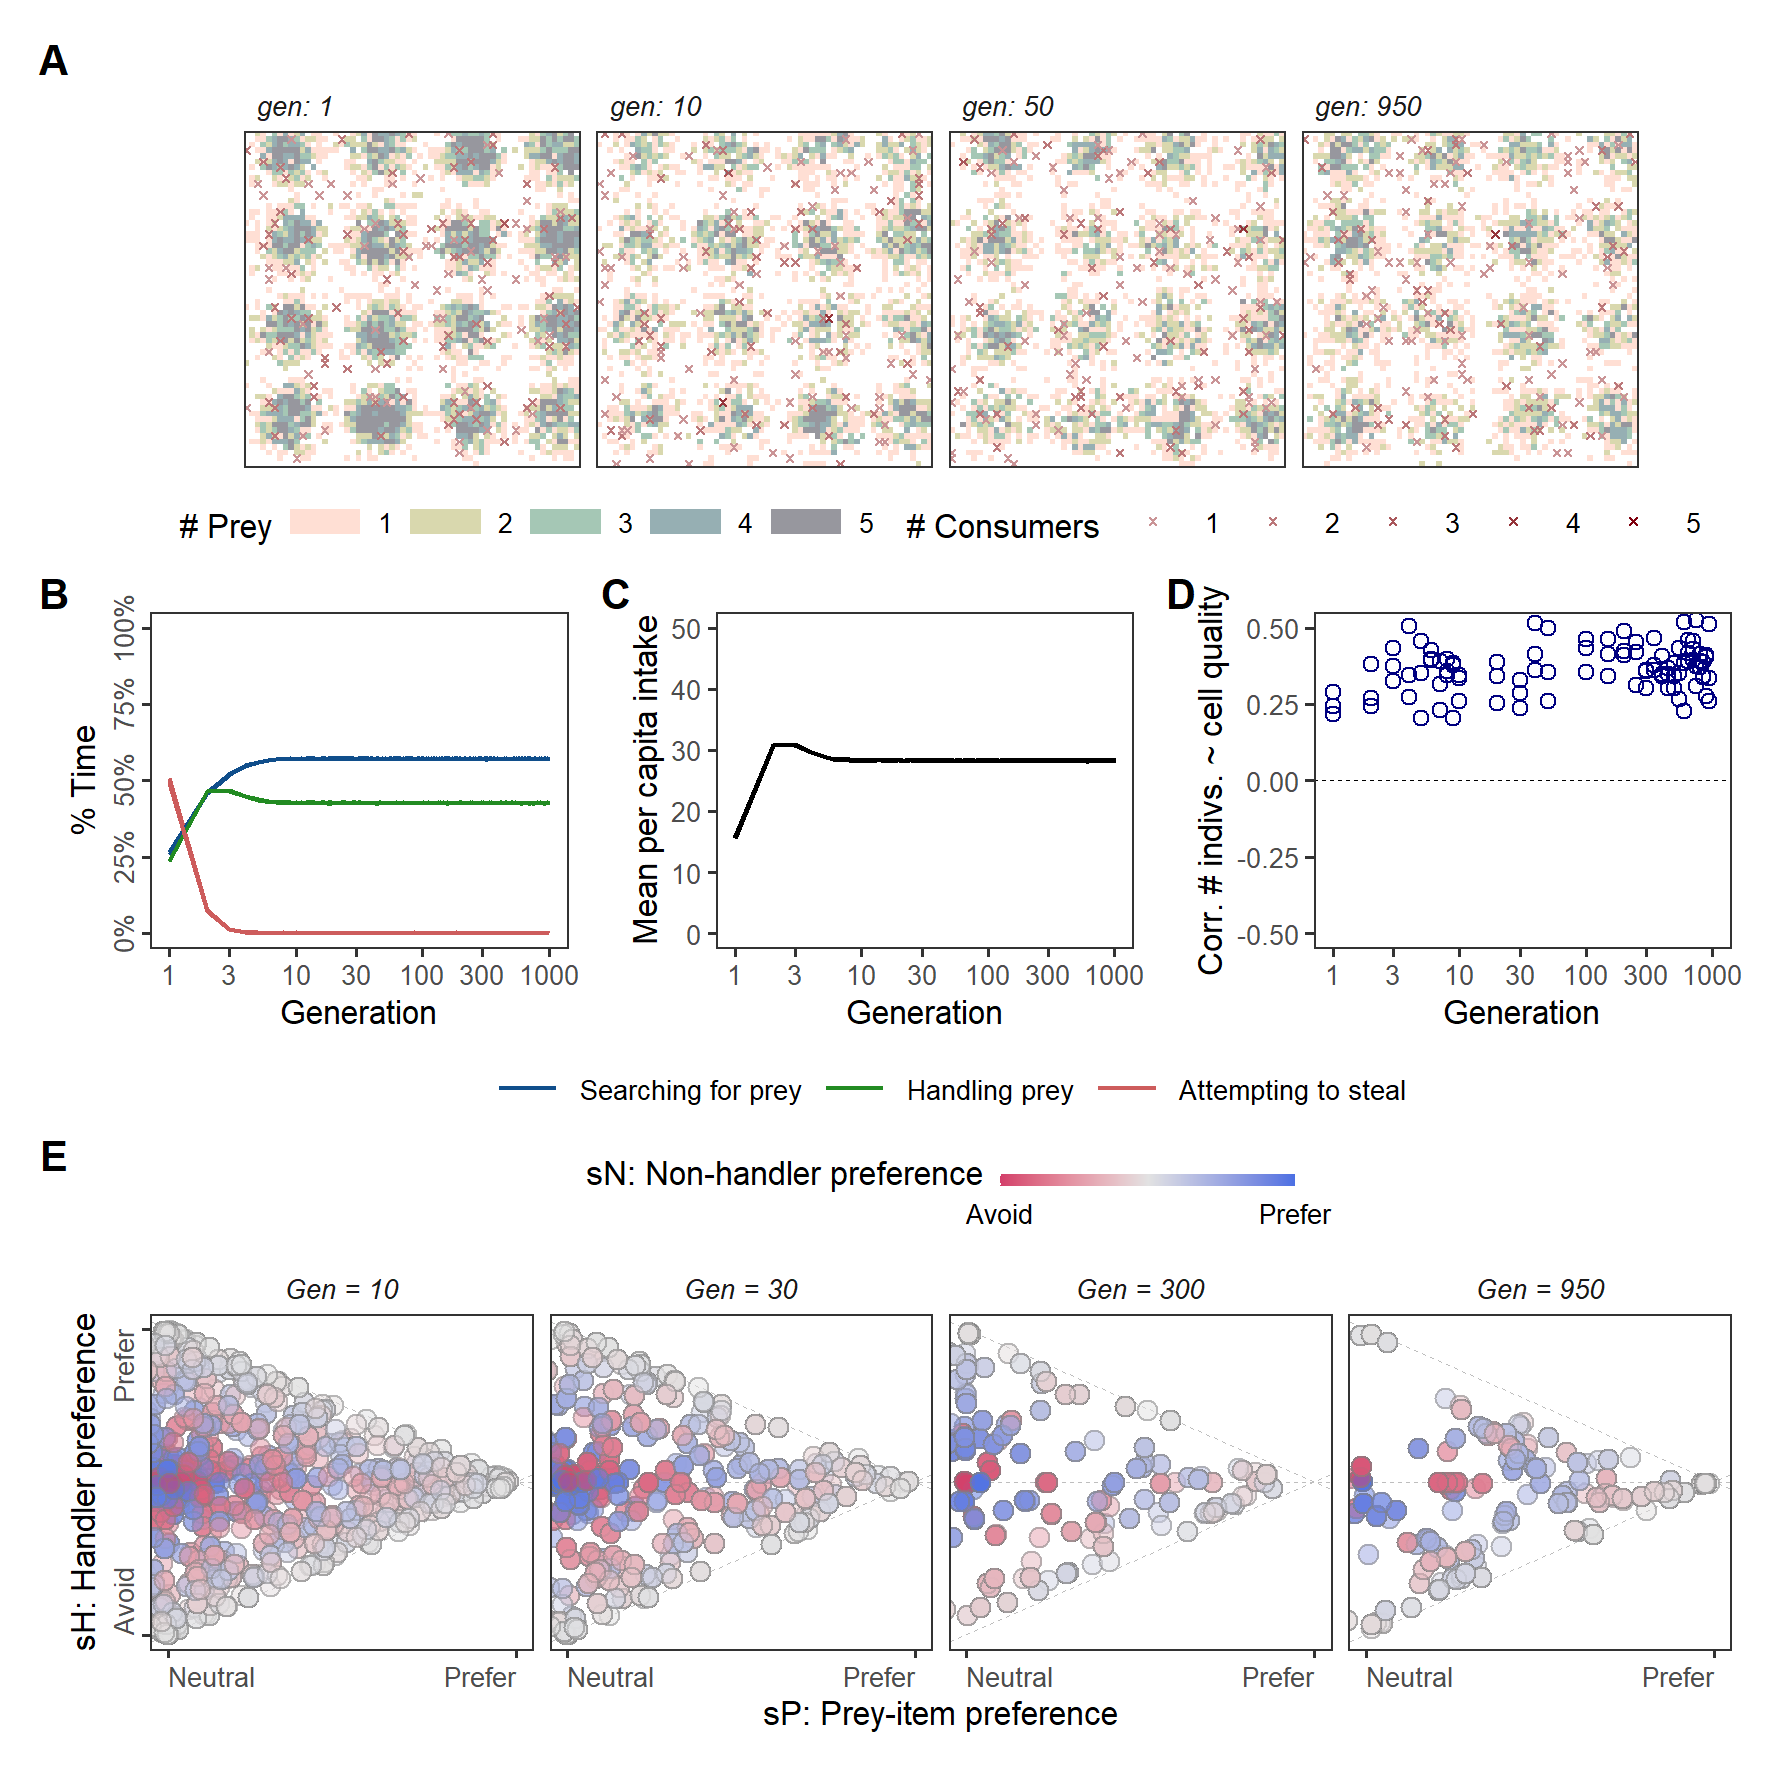
\includegraphics{"figures/fig_0random.png"}
\caption{\textbf{The evolutionary ecology of random movement serves as a useful baseline against which to compare other scenarios}. \textbackslash{}textbf\{(A)\} Individuals deplete the landscape (\(r_{max}\) = 0.01) at random, allowing it to regenerate more than scenario 1, yet less than scenario 2. \textbackslash{}textbf\{(B)\} Kleptoparasitism as a strategy very rapidly goes extinct, as individuals cannot move towards handlers, and encountering a handler at random is very unlikely. \textbackslash{}textbf\{(C)\} Surprisingly, moving at random yields a similar mean per-capita intake as in scenarios 1 and 3, and actually better than scenario 2. \textbackslash{}textbf\{(D)\} Random movement leads, unsurprisingly, to no correlation with landscape productivity. \textbackslash{}textbf\{(E)\} When movement strategies are not under selection, individuals occupy a large area of the potential strategy space, including negative values of \(s_P\) (which is not shown here).}
\end{figure}

\newpage

\hypertarget{evolution-of-movement-strategies-across-replicates}{%
\section{Evolution of Movement Strategies Across Replicates}\label{evolution-of-movement-strategies-across-replicates}}

\begin{figure}
\centering
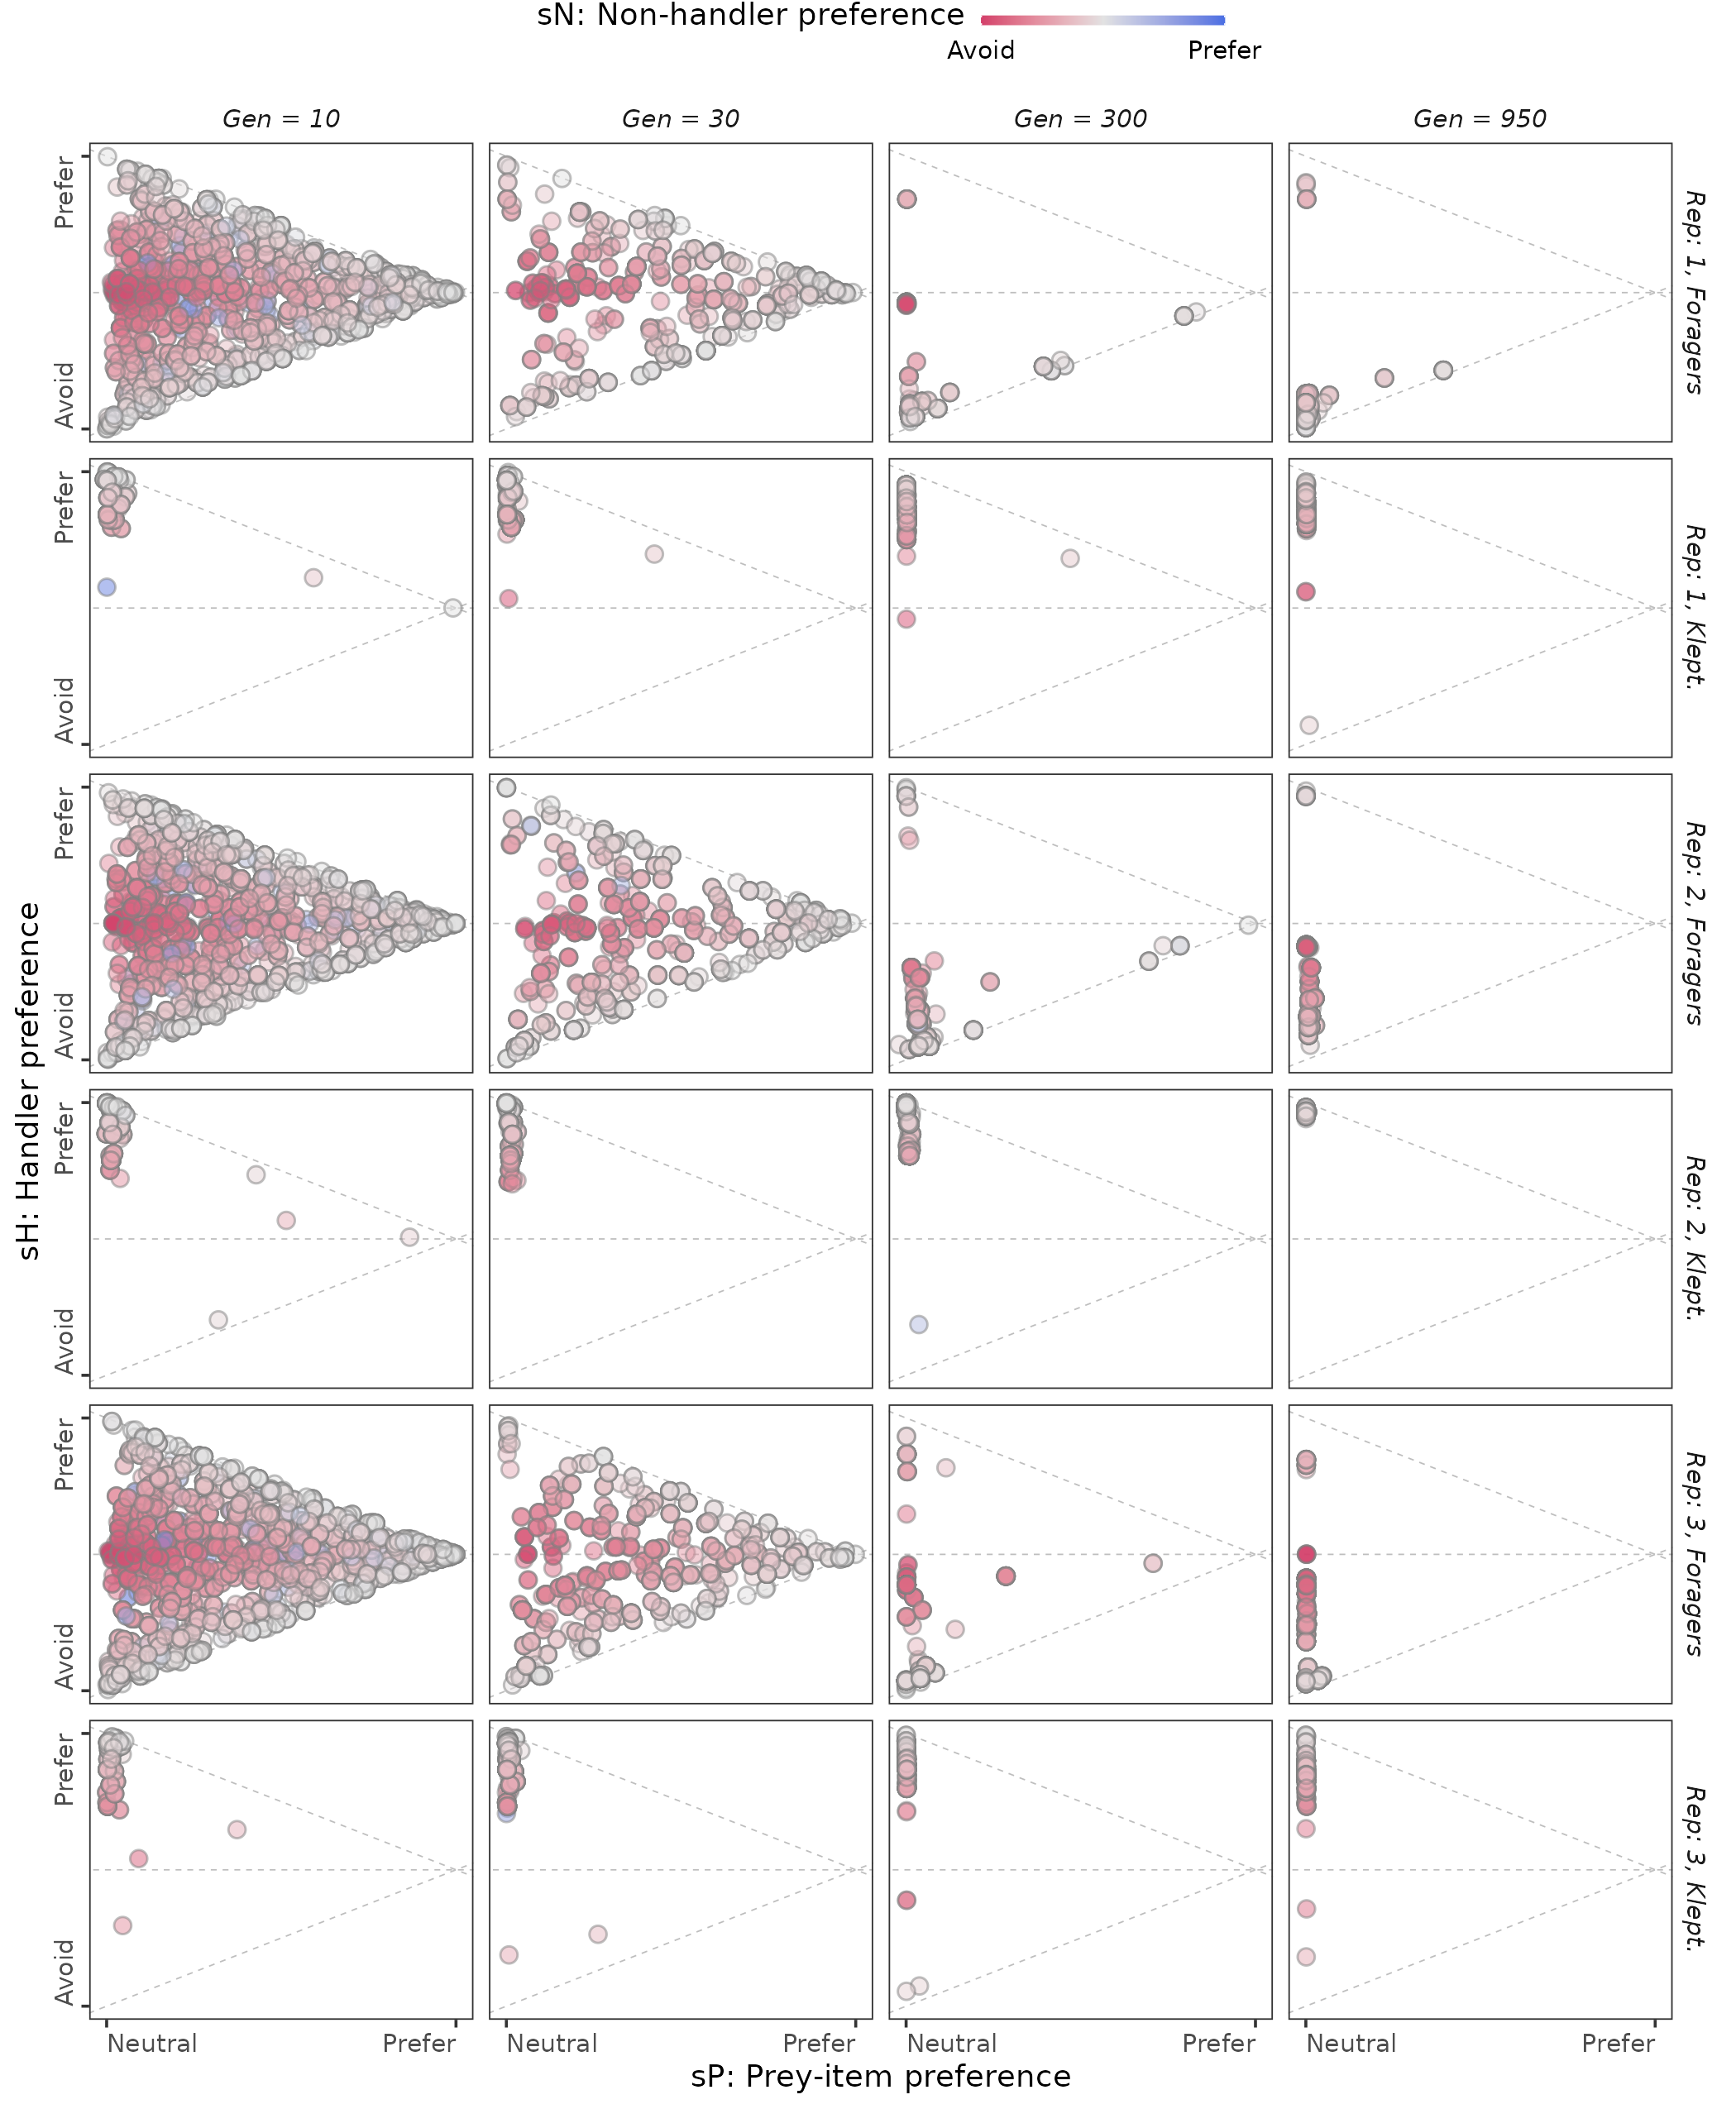
\includegraphics[width=0.8\textwidth,height=\textheight]{"figures/fig_wt_evo_sc_obligate.png"}
\caption{\textbf{Evolution of movement strategies in scenario 2}. Across simulation replicates (\(r_{max}\) = 0.01), in populations with fixed forager or kleptoparasite strategies, the two competition strategies consistently undergo rapid evolutionary divergence in movement strategies. Kleptoparasites evolve within 10 generations to primarily track handlers, and maintain this preference across hundreds of generations. Foragers are slower to converge upon a single movement strategy, but eventually (G = 300) mostly avoid handlers and non-handlers alike. A small fraction of both kleptoparasites and foragers have the strategy correlated with the opposite competition strategy, likely due to mutation in the competition strategy.}
\end{figure}

\begin{figure}
\centering
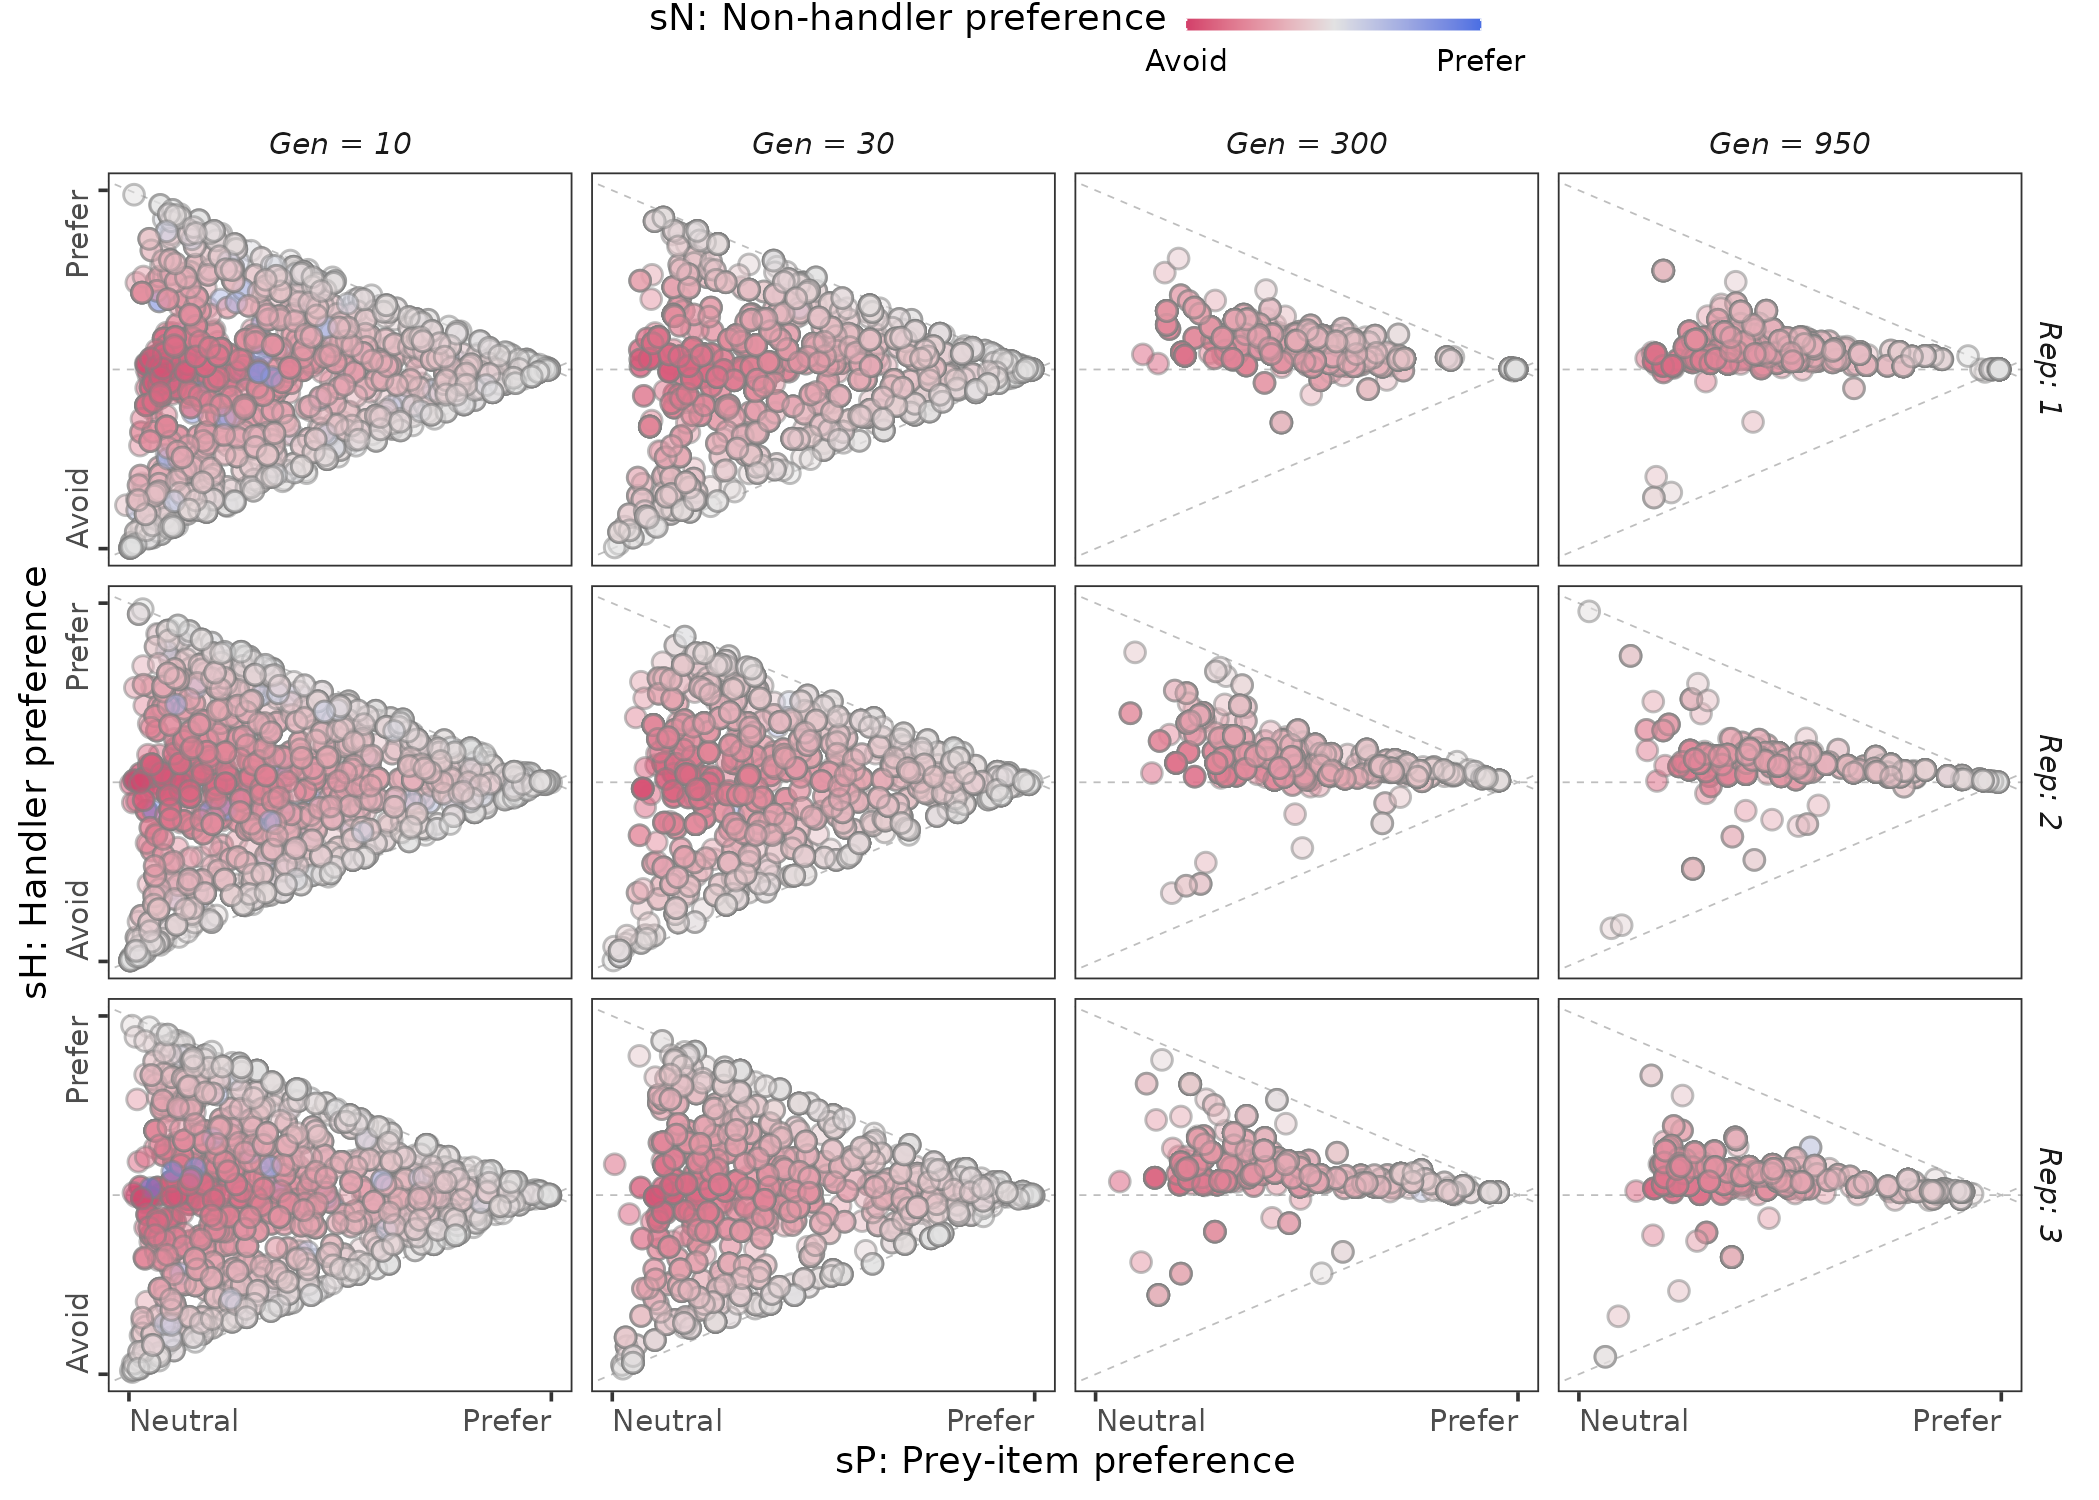
\includegraphics[width=0.8\textwidth,height=\textheight]{"figures/fig_wt_evo_sc_foragers.png"}
\caption{\textbf{Evolution of movement strategies in scenario 1}. Across simulation replicates (\(r_{max}\) = 0.01), populations of foragers consistently evolve a wide range of movement strategies to move towards prey items, largely move towards successful foragers (handlers), and avoid unsuccessful foragers (non-handlers).}
\end{figure}

\begin{figure}
\centering
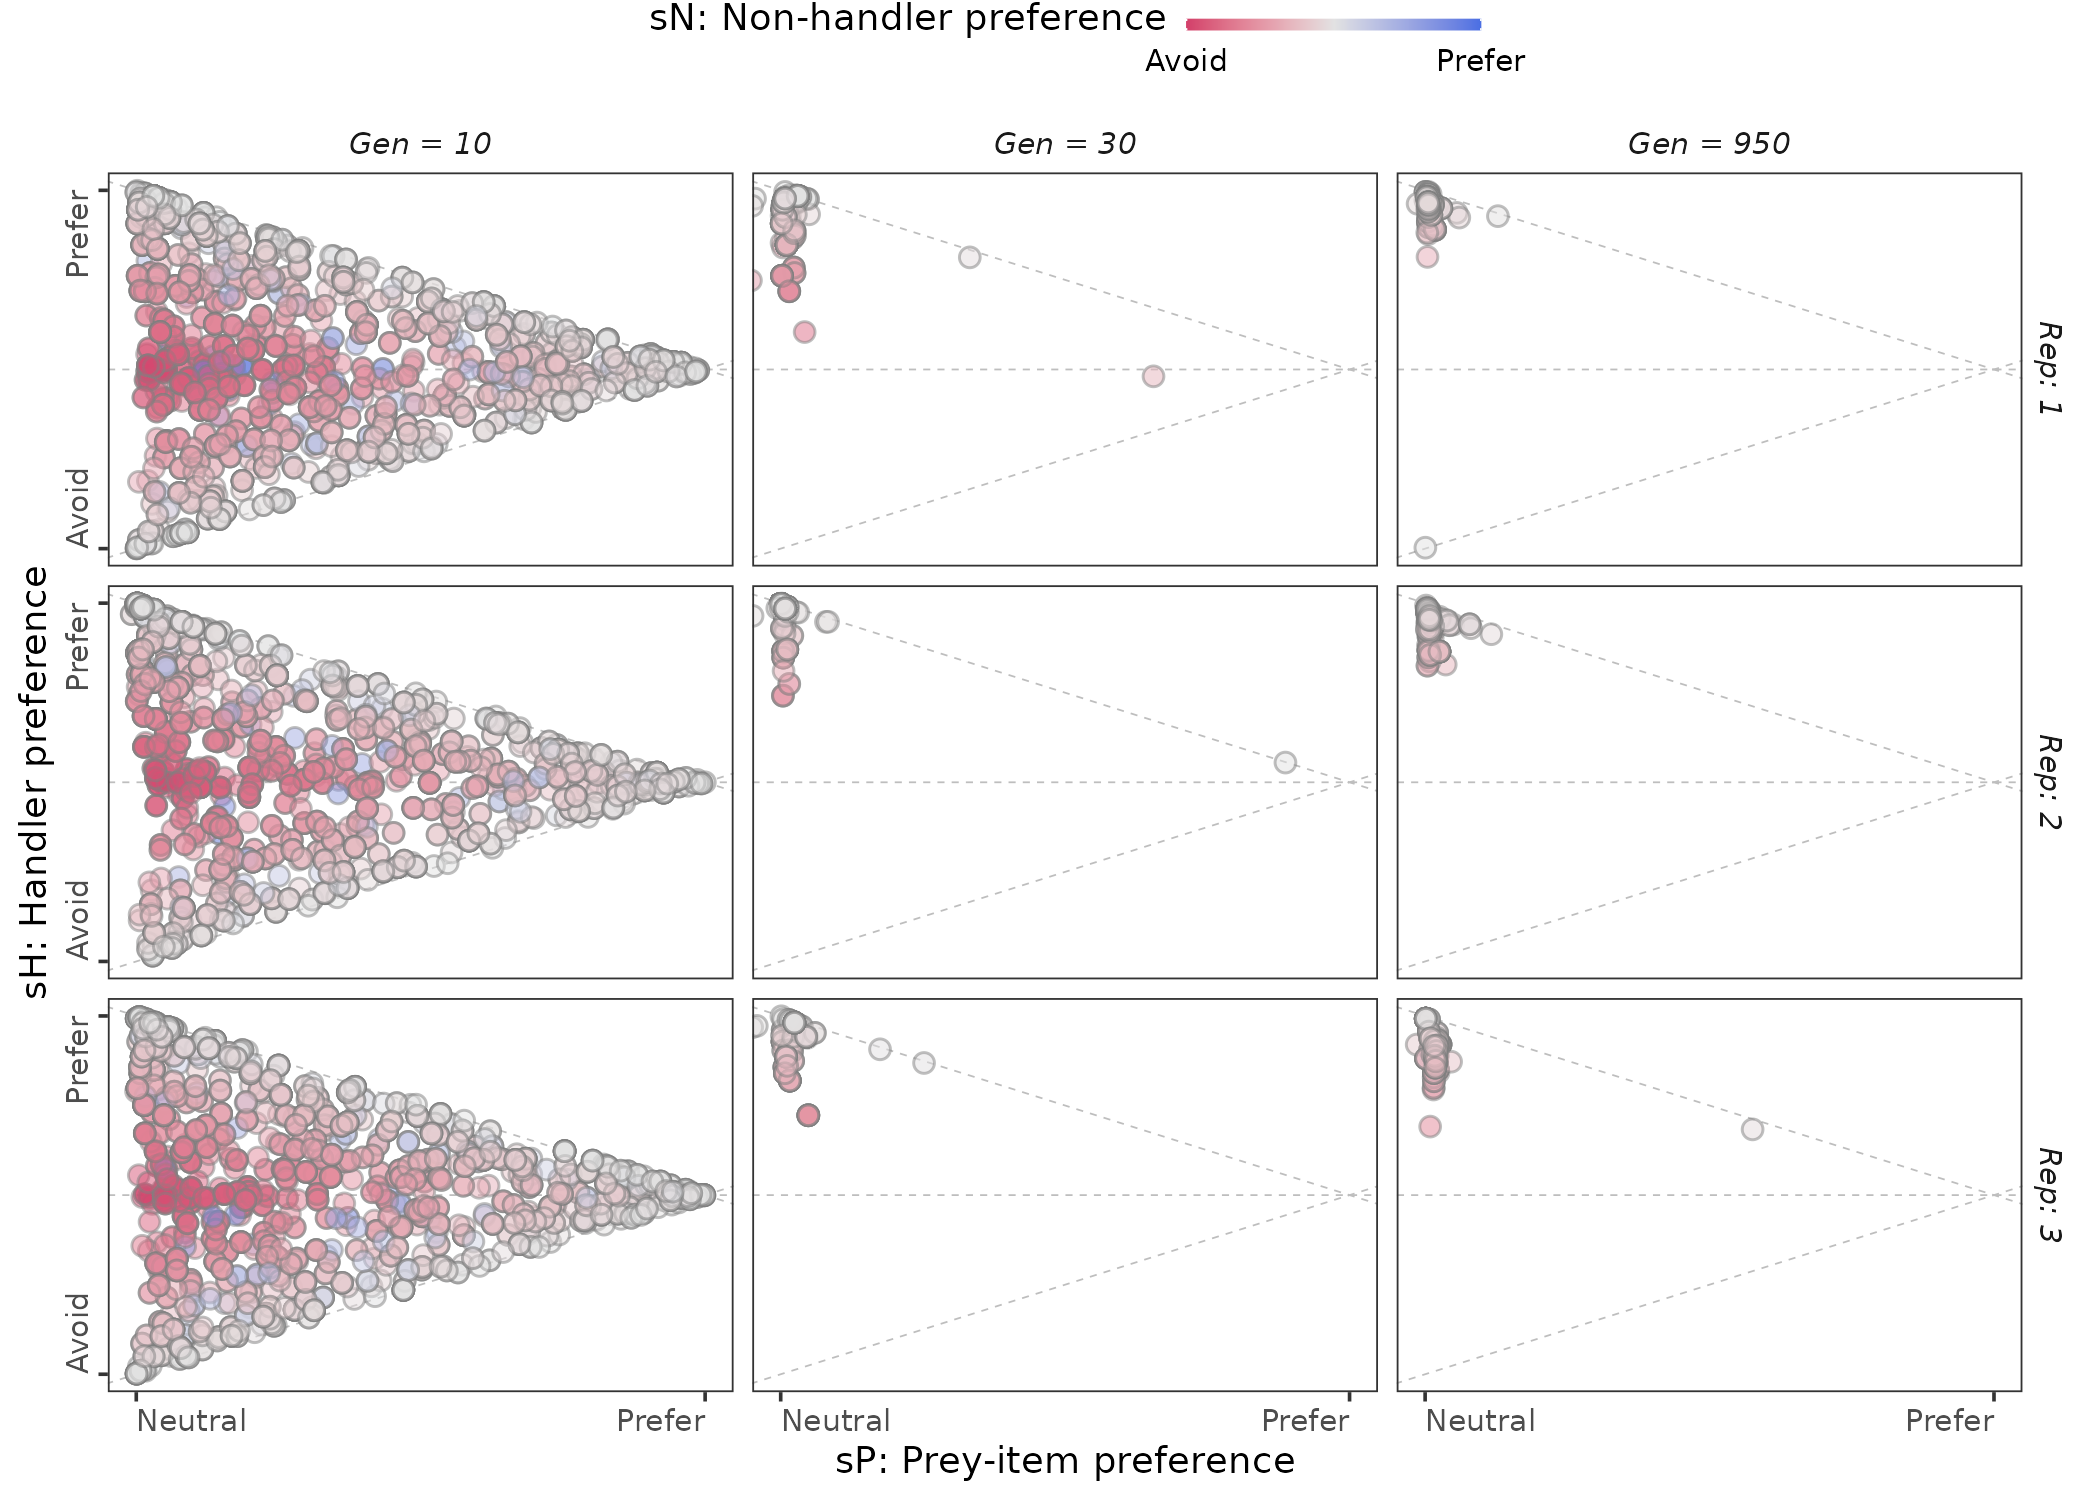
\includegraphics[width=0.8\textwidth,height=\textheight]{"figures/fig_wt_evo_sc_facultative.png"}
\caption{\textbf{Evolution of movement strategies in scenario 3}. Across simulation replicates (\(r_{max}\) = 0.01), populations of consumers that choose their competition strategy using inherited preferences, consistently evolve to move primarily towards handlers, a strategy that facilitates kleptoparasitism.}
\end{figure}

\newpage

\hypertarget{individual-differences-in-movement-strategies-in-scenarios-2-and-3}{%
\section{Individual Differences in Movement Strategies in Scenarios 2 and 3}\label{individual-differences-in-movement-strategies-in-scenarios-2-and-3}}

\begin{figure}
\centering
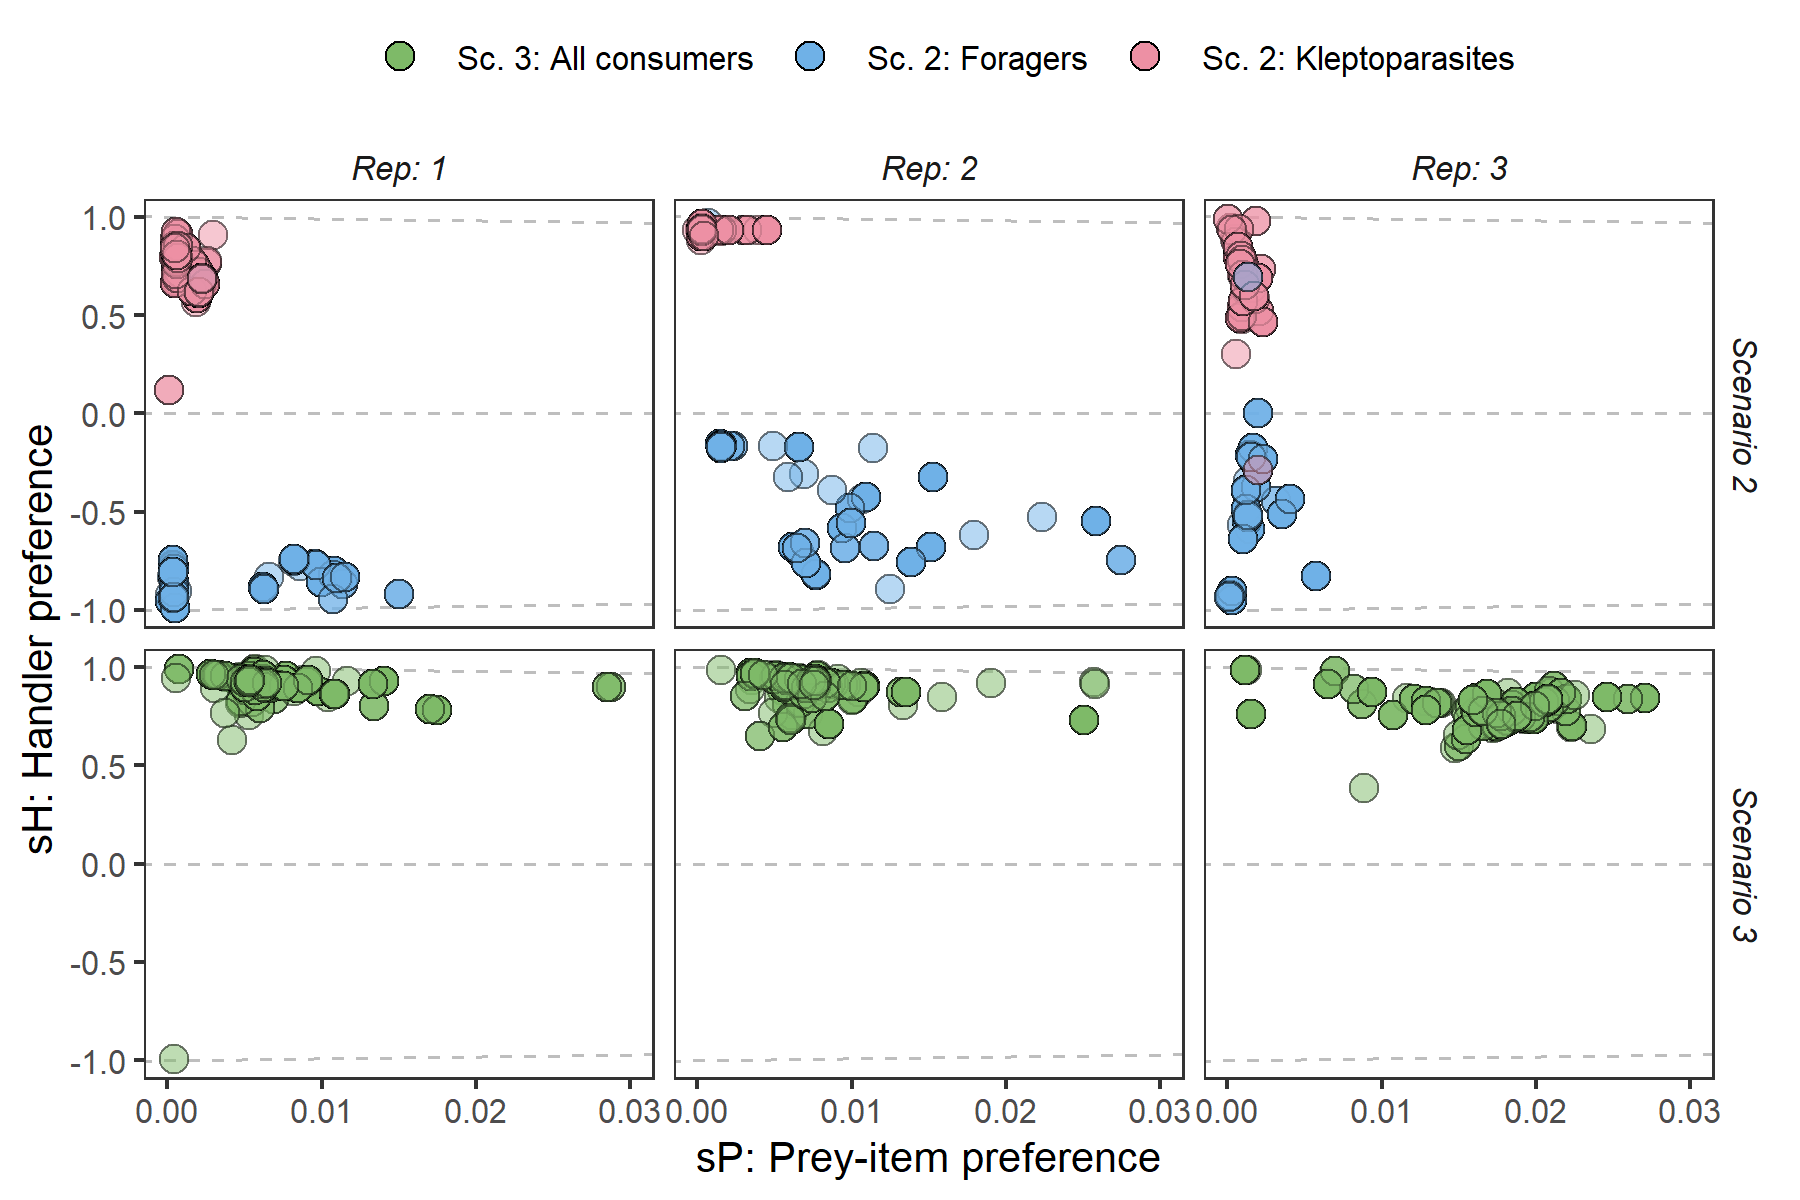
\includegraphics{"figures/fig_small_scale_variation.png"}
\caption{\textbf{Small-scale individual variation may be hidden by primary drivers of behaviour}. Across simulation replicates (\(r_{max}\) = 0.01), populations in scenarios 2 and 3 do show small-scale individual variation in preference for prey density cues (\(s_P\)). This variation is unlikely, in our model, to lead to functional differences in movement paths, but may cause very small emergent differences in model implementations of movement over a continuous space. It is key therefore to measure variation, and the relative contribution of such variation, along multiple axes of behaviour when studying the functional consequences of individual differences.}
\end{figure}

\newpage

\hypertarget{evolution-of-and-variation-in-competition-strategies-in-scenario-3}{%
\section{Evolution of, and Variation in Competition Strategies in Scenario 3}\label{evolution-of-and-variation-in-competition-strategies-in-scenario-3}}

\begin{figure}
\centering
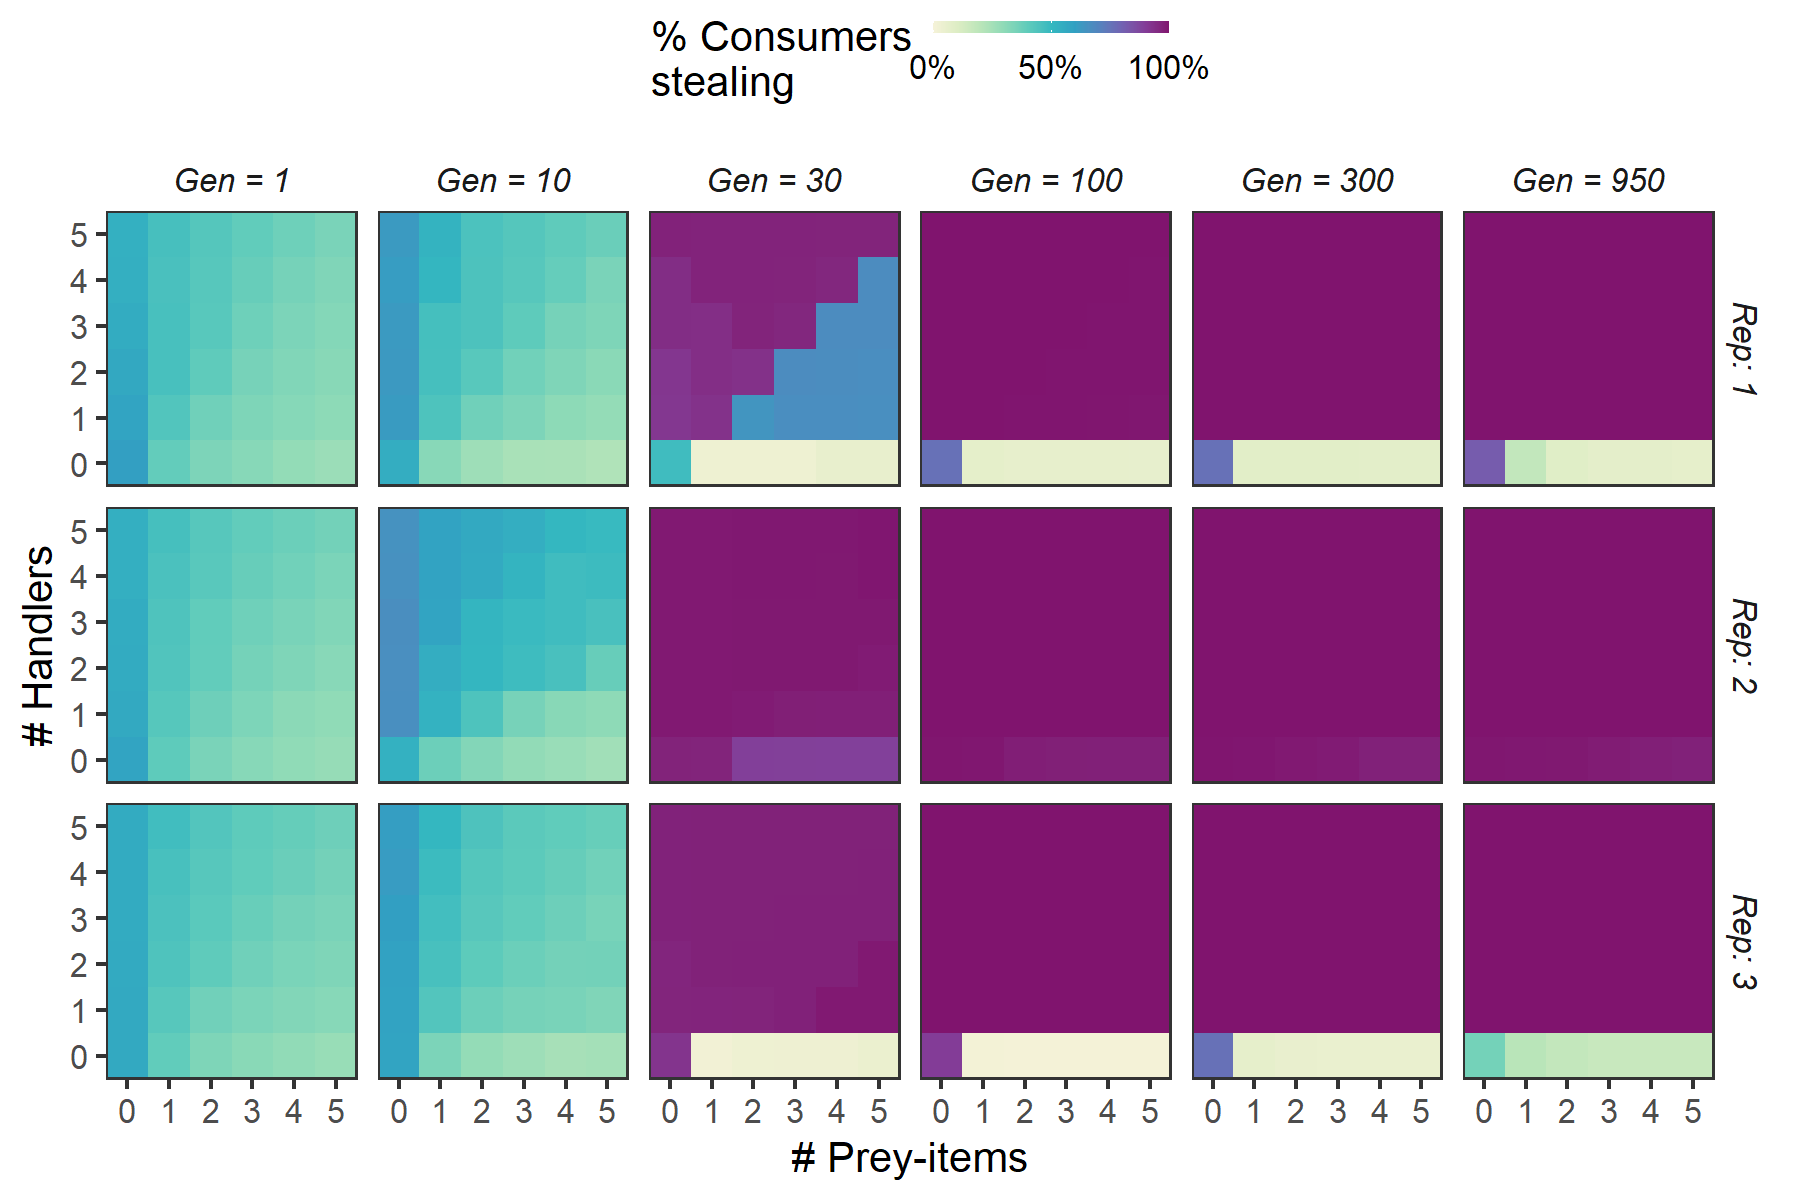
\includegraphics{"figures/fig_sc3_comp_evol.png"}
\caption{\textbf{Evolution of conditional kleptoparasitic behaviour in scenario 3.} Across replicates in scenario 3, individuals rapidly evolve conditional competition strategies that lead them to attempt to steal across a wide range of ecological conditions. Mainly, within 100 generations (and in some cases, only 30 generations), all individuals choose a kleptoparasitic strategy when handlers are available, even if there are multiple food items also available. Only when there are no handlers, do most individuals choose to forage for prey, with more individuals choosing to forage as prey density increases. Surprisingly, when there is no information, most individuals in later generations adopt a kleptoparasitic strategy by default. Replicate 2 shows why this is an incomplete assessment of individuals' competitive choices: all individuals appear to choose to steal regardless of ecological cues, with this strategy apparently persisting across many generations. This would lead to no intake at all, and no such drop is seen in mean per-capita intake. This points to the likely role of unsuccessful consumers, non-handlers, in determining competition strategy in this scenario.}
\end{figure}

\newpage

\hypertarget{effect-of-landscape-productivity-r_max-on-resource-landscape-depletion}{%
\section{\texorpdfstring{Effect of Landscape Productivity (\(r_{max}\)) on Resource Landscape Depletion}{Effect of Landscape Productivity (r\_\{max\}) on Resource Landscape Depletion}}\label{effect-of-landscape-productivity-r_max-on-resource-landscape-depletion}}

\begin{figure}

{\centering \includegraphics[width=\textwidth]{supplementary_material_files/figure-latex/unnamed-chunk-15-1} 

}

\caption{In scenario 1, foragers completely deplete the resource landscape within 10 generations at low $r_{max}$ (A, B). However, at $r_{max} >$ 0.01 (C, D), prey item regeneration exceeds depletion and the resource landscape is rapidly saturated until most cells carry 5 items, the maximum allowed in our model.}\label{fig:unnamed-chunk-15}
\end{figure}

\begin{figure}

{\centering \includegraphics[width=\textwidth]{supplementary_material_files/figure-latex/unnamed-chunk-16-1} 

}

\caption{In scenario 2, foragers can only deplete the resource landscape at very low $r_{max}$ (A): 1 prey item generated per 1,000 timesteps, or 2.5 generations. At all $r_{max} \geq$ 0.05 (B, C, D), prey item regeneration matches or exceeds depletion and the resource landscape either shows strong spatial structure, or is entirely saturated with prey items.}\label{fig:unnamed-chunk-16}
\end{figure}

\begin{figure}

{\centering \includegraphics[width=\textwidth]{supplementary_material_files/figure-latex/unnamed-chunk-17-1} 

}

\caption{Scenario 3 is similar to scenario 1 at low $r_{max}$ (A, B), where foragers completely deplete the resource landscape). Similarly, at $r_{max} >$ 0.01 (C, D), prey item regeneration exceeds depletion and the resource landscape is rapidly saturated to a carrying capacity of 5 prey items per cell.}\label{fig:unnamed-chunk-17}
\end{figure}

\end{document}
